\newpage
\section{Durchführung}
\label{sec:Durchführung}

\subsection{Aufbau des \ce{Ge}-Detektors}
\label{sec:AufbauDetektor}

Der verwendete Detektor ist ein sogenannter koaxialer \ce{Ge}-Detektor.
Er besteht aus einem zylinderförmigen \ce{Ge}-Kristall mit einer Bohrung in
Inneren, auf welche ein Kontakt aufgedampft ist. Von außen sind \ce{Li}-Atome
eindiffundiert, sodass die äußere Schicht von \SI{0.5}{\milli\meter} Dicke
stark n-dotiert ist.
Zwischen den Goldkontakt und die äußere dotierte Schicht lässt sich eine äußere
Spannung $U$ anlegen.
Zur Abschirmung des Detektors ist dieser Aufbau von einer Aluminium-Schutzhaube
umgeben. Als Konsequenz existiert eine untere Nachweisgrenze für $\gamma$-Quanten
von \SIrange{40}{50}{\kilo\electronvolt}.
Dieser Aufbau ist in Abbildung \ref{fig:Versuchsaufbau} dargestellt.
Hierbei strahlt die Quelle von oben auf den Detektor.
Die Aluminium-Schutzhaube sitzt wiederum auf der Spitze eines mit flüssigem
Stickstoff gefülltem Dewargefäß. Die Kühlung erfolgt über einen wärmeleitenden
Kühlfinger, über welchen das Stickstoffreservoir und der Kristall in Verbindung stehen.
Der gesamte Aufbau befindet sich in einer Bleiverkleidung, um die Detektion
von Hintergrundstrahlung zu verhindern. Innerhalb befindet sich weiterhin eine
Platte aus hochreinem Kupfer, welche die natürliche Strahlung des Bleis vor dem
Detektor abschirmt.
\begin{figure}
	\centering
	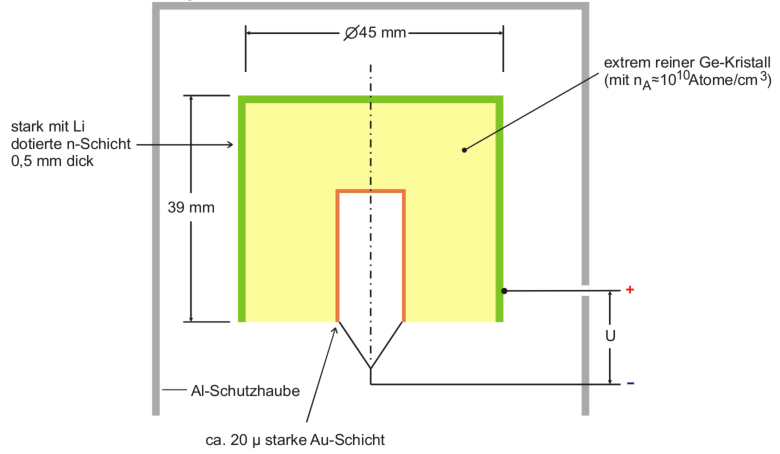
\includegraphics[width=.8\textwidth]{images/Versuchsaufbau.pdf}
	\caption{Schematische Darstellung eines koaxialen Reinst-\ce{Ge}-Detektors~\cite[14]{anleitung}.}
	\label{fig:Versuchsaufbau}
\end{figure}

Um von dem aufgenommenen Spektrum auf die Aktivität nach Formel \eqref{eqn:Vollenergie-Nachweiseffizienz}
schließen zu können, wird der Raumwinkel benötigt.
Da der Abstand $a$ zwischen Quelle und Detektor groß gegenüber der Quellenabmessung
ist, gilt der Zusammenhang
\begin{equation}
	\frac{\Omega}{2\:\pi} = \frac{1}{2} \left(1 - \frac{a}{\sqrt{a^2 + r^2}}\right)
	\label{eqn:Raumwinkel}
\end{equation}
mit dem Radius $r$ nach Abbildung \ref{fig:Raumwinkel}.
\begin{figure}
	\centering
	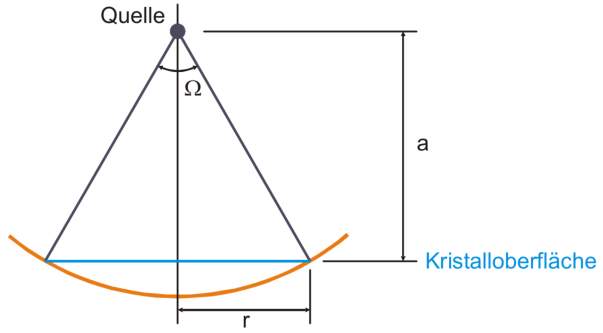
\includegraphics[width=.5\textwidth]{images/Raumwinkel.pdf}
	\caption{Skizze zur Berechnung des Raumwinkels $\Omega$~\cite[25]{anleitung}.}
	\label{fig:Raumwinkel}
\end{figure}

\subsection{Beschaltung des Detektors}
\label{sec:Schaltungen}

Der Detektor ist an eine elektronische Schaltung angeschlossen, die eine Überführung
der Strompulse des Detektors in Spannungspulse ermöglicht und diese nach Pulshöhe sortiert.
Diese Schaltung ist schematisch in Abbildung \ref{fig:Gesamtschaltbild} dargestellt.
\begin{figure}
	\centering
	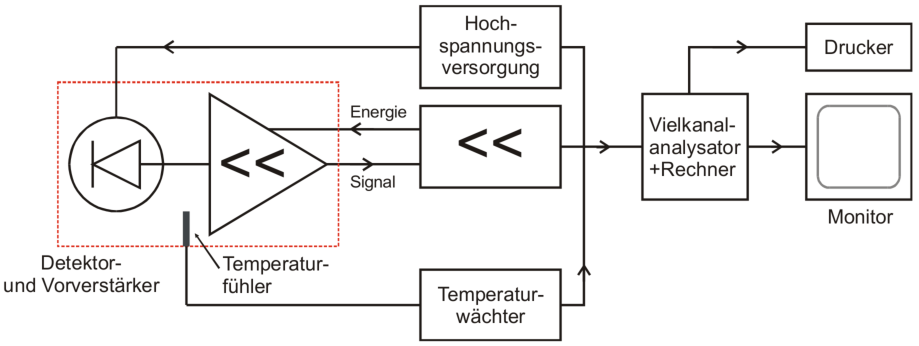
\includegraphics[width=.9\textwidth]{images/Gesamtschaltbild.pdf}
	\caption{Schematische Darstellung der elektronischen Beschaltung des Detektors~\cite[22]{anleitung}.}
	\label{fig:Gesamtschaltbild}
\end{figure}
Wie in Abschnitt \ref{sec:KenngroessenHLDetektor} angedeutet befindet sich ein Vorverstärker
innerhalb des Dewargefäßes, welchen den Detektor kühlt, um Rauschspannungen zu minimieren.
Ein Temperaturfühler im Inneren des Dewargefäßes ist mit einem Temperaturwächter verbunden,
welcher das Anlegen einer Hochspannung an einen warmen Detektorkristall verhindert.
Der Vorverstärker besteht aus einem kapazitiv rückgekoppleten Operationsverstärker, sodass
das Ausgangspotential proportional zum integrierten Eingangsstrom ist.
Dies führt beim Einfall mehrerer $\gamma$-Quanten zu einem stufenförmigen Anstieg der Ausgangsspannung.
Aus diesem Signal ist eine Analyse der Pulshöhen schwierig,
sodass der Integrationskondensator $C_\text{k}$ durch eine optoelektronische Rückkopplung
entladen wird. In Abbildung \ref{fig:Optoelektronische-Rueckkopplung} ist das Schaltbild
des Operationsverstärkers mit Rückkopplung dargestellt.
\begin{figure}
	\centering
	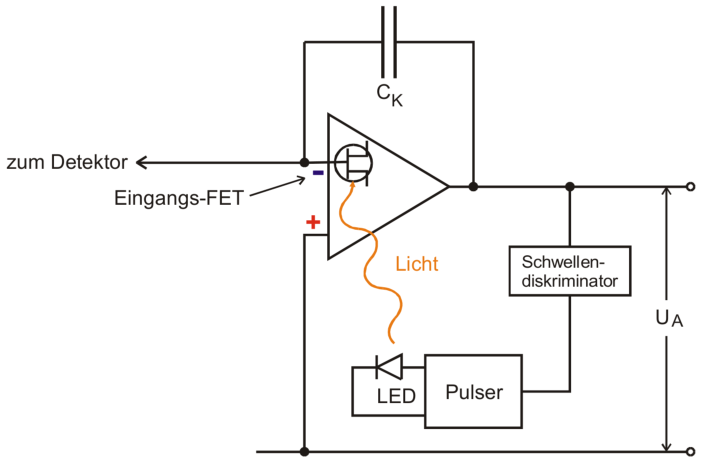
\includegraphics[width=.7\textwidth]{images/Optoelektronische-Rueckkopplung.pdf}
	\caption{Schematisches Schaltbild des Vorverstärkers mit optoelektronischer Rückkopplung~\cite[19]{anleitung}.}
	\label{fig:Optoelektronische-Rueckkopplung}
\end{figure}
Nach einem Impuls scheint eine LED auf den Eingangs-Feldeffekttransistor, welcher so kurzzeitig
leitend wird und eine Entladung des Kondensators ermöglicht.
Der Vorvertärker ist über einen Hochpass an den Hauptverstärker gekoppelt, um Gleichspannungsdriften
und Offsetspannung nicht zu verstärken. Aufgrund unterschiedlicher Abklingkoeffizienten des
Hochpasses und der kapazitiven Rückkopplung des Operationsverstärkers kann es zu sogenannten
Unterschwingern kommen, durch welche das Ausgangssignal zeitweise kleiner als Null ist. Dies
wird durch sogenannte Zero-Pole-Kompensation unterbunden, also das geben eines geeigneten
Bruchteils der Ausgangsspannung des Vorverstärkers auf den Hauptverstärker bei Umgehung
des Hochpasses.
Im Hauptverstärker selbst wird das Signal mehrfach elektronisch integriert und differenziert,
um eine optimale Bandbreite des Verstärkers zu gewährleisten. Bei zu kleiner Bandbreite werden
werden nicht alle Komponenten des Eingangssignals übertragen und bei zu großer Bandbreite
ist das Signal zu Rauschverhältnis zu klein.

Nach Verstärkung des Signals wird die Pulshöhe mit einem Wilkinson-Analog-Digital-Konverter
gemessen, dessen Schaltbild in Abbildung \ref{fig:Wilkinson-Analog-Digital-Konverter} dargestellt ist.
\begin{figure}
	\centering
	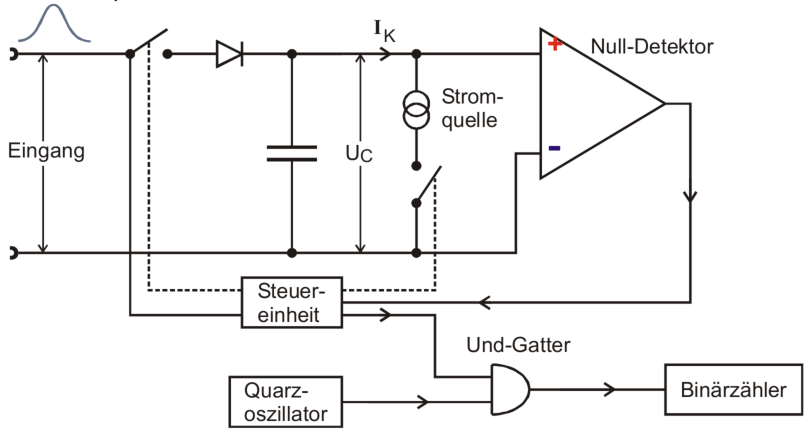
\includegraphics[width=.8\textwidth]{images/Wilkinson-AD-Konverter.pdf}
	\caption{Schaltbild eines Wilkinson-Analog-Digital-Konverters~\cite[21]{anleitung}.}
	\label{fig:Wilkinson-Analog-Digital-Konverter}
\end{figure}
Ein Eingangsimpuls lädt einen Kondensator auf. Im Anschluss schließt verhindert eine Steuereinheit
das Aufladen durch weitere Impulse, bis dieser Impuls ausgelesen wurde.
Währenddessen wird der Kondensator über eine Stromquelle entladen, bis ein Null-Detektor eine
Entladung des Kondensators feststellt. In der Entladezeit wird die Anzahl an Impulsen eines
hochstabilen Quarz-Oszillators bestimmt, sodass die Zahl des Binärzählers proportional zur
Pulshöhe des Eingangsimpulses ist.
Während der Entladezeit ist die Aufnahme eines weiteren Eingangsimpulses nicht möglich,
sodass der Konverter eine Totzeit von typischerweise $\sim \SI{40}{\micro\second}$ aufweist.
Die erhaltene Binärzahl wird an einen Vielkanal-Analysator weiter gegeben, welcher
die Anzahl an Pulsen in Abhängigkeit von den Pulshöhen speichert und auf einem angeschlossenem
Bildschirm ausgibt.

\subsection{Kalibrierung des Detektors}
\label{sec:KalibrierungBeschreibung}

Zuerst wird der Verstärker eingeschaltet und geprüft, ob der Detektor gekühlt ist.
Im Anschluss wird langsam die eine äußere Spannung von \SI{5}{\kilo\volt} angelegt
und der Abstandshalter mit einer Schieblehre vermessen,
welcher den Abstand zwischen Probe und Detektor festlegt.
Im Anschluss wird das Spektrum eines kalibrierten \ce{^125Eu}-Strahlers für eine Stunde aufgenommen.
Hieraus lässt sich die Energieeichung und Vollenergie-Nachweiseffizienz
des Detektors bestimmen.
Die theoretischen Emissionswahrscheinlichkeiten sind dazu in \cite[28]{anleitung} angegeben.
Die Aufnahme des Spektrums erfolgt mit Hilfe des Computerprogramms
\texttt{MAESTRO} und die erhaltenen Spektren werden als ASCII-Dateien gespeichert.

Im Anschluss wird die Europium-Probe entfernt und ein \ce{^137Cs}-Strahler eingesetzt,
um weitere Detektoreigenschaften wie die Absorptionswahrscheinlichkeit für
\ce{^137Cs}-Quanten zu bestimmen.
Hier beträgt die Messzeit ebenfalls eine Stunde.

\subsection{Charakterisierung unbekannter Proben}
\label{sec:CharakterisierungBeschreibung}

Die dritte Probe ist entweder eine \ce{^125Sb}- oder eine \ce{^133}-Quelle.
Das Spektrum wird wie auch bei der vierten Probe für eine Stunde aufgenommen
und daraus im Anschluss das vorliegende Material bestimmt.
Hierzu werden Tabellen mit verschiedenen $\gamma$-Linien und den zugehörigen
Emissionswahrscheinlichkeiten für Barium und Antimon aus \cite[28]{anleitung}
verwendet.
Die vierte Quelle ist ein unbekannter Strahler, dessen Zusammensetzung
aus dem Spektrum ermittelt werden soll.
